\documentclass[runningheads,envcountsame]{llncs}
\usepackage{amsmath,amsfonts, amssymb, mathtools,stackrel}
\usepackage[usenames]{color}
\usepackage[dvipsnames]{xcolor}
\usepackage{colortbl}
\usepackage{algorithm}
\usepackage[noend]{algpseudocode}
\usepackage[lambda, advantage ,operators, sets,adversary,landau,probability,notions,logic,ff,mm,primitives,events,complexity,asymptotics,keys]{cryptocode}
\usepackage{comment}
\usepackage{numprint}
\usepackage{mdframed}
\npthousandsep{\,}
\usepackage{tikz-cd}
\definecolor{NTNUBlue}{HTML}{00509e}
\usepackage[bookmarks,bookmarksdepth=2,pdfusetitle,colorlinks,linkcolor=NTNUBlue,citecolor=NTNUBlue,urlcolor=NTNUBlue]{hyperref}

\usepackage[nameinlink]{cleveref}
\usepackage{multirow}

\usepackage{todonotes}

 \spnewtheorem{plaindef}[theorem]{Definition}{\bfseries}{}
%notes
\newcommand{\mattia}[1]{\hspace*{0,01pt}\todo[color=NTNUBlue!40]{#1}}
\definecolor{darkgreen}{rgb}{0,0.5,0}
\newcommand{\jiaxin}[1]{\hspace*{0,01pt}\todo[color=darkgreen!40]{#1}}


%fonts
\newcommand{\setfont}[1]{\mathcal{#1}}
\newcommand{\algfont}[1]{{\mathsf{#1}}}
\newcommand{\mathsc}{\textsc}
%code
\newcommand{\getsr}{\gets_{\scriptscriptstyle\$}} %dollar behind arrow
\renewcommand{\getsr}{\mathrel{\vbox{\offinterlineskip\ialign{
				\hfil##\hfil\cr
				\hspace{0.1em}$\scriptscriptstyle\$$\cr
				$\leftarrow$\cr
}}}} %dollar on arrow
\def\makeuppercase#1{
	\expandafter\newcommand\csname cal#1\endcsname{\mathcal{#1}}
	\expandafter\newcommand\csname adv#1\endcsname{\mathcal{#1}}
	\expandafter\newcommand\csname frak#1\endcsname{\mathfrak{#1}}
	\expandafter\newcommand\csname bb#1\endcsname{\mathbb{#1}}
	\expandafter\newcommand\csname bf#1\endcsname{\textbf{#1}}
}
\newcounter{char}
\setcounter{char}{1}
\loop
\edef\Letter{\Alph{char}}
\expandafter\makeuppercase\Letter
\stepcounter{char}
\unless\ifnum\thechar>26
\repeat
%spaces
\newcommand{\Domain}{\mathcal{D}}
\newcommand{\Codomain}{\mathcal{C}}
\newcommand{\Language}{\mathcal{L}}
\newcommand{\PKSpace}{\mathcal{PK}}
\newcommand{\SKSpace}{\mathcal{SK}}
\newcommand{\changehighlight}[1]{#1}

%roles
\newcommand{\Universe}{\mathcal{U}}
\newcommand{\Party}{\mathsf{P}}
\newcommand{\PartySet}{\setfont{P}}
\newcommand{\User}[1][]{\Party_{#1}}
\newcommand{\GakePk}[1][]{\spk_{#1}}
\newcommand{\GakeSk}[1][]{\ssk_{#1}}
\newcommand{\attack}{\text{attack}}
\newcommand{\matchingSessions}{\mathfrak{M}(\sID^*)}
\newcommand{\suchthat}{\text{ s.\,t. }}
\newcommand{\pcor}{\textbf{or }}
\newcommand{\tabfalse}{$\mathbf{F}$}
\newcommand{\pcfetch}{\textbf{fetch} }
\newcommand{\pcbroadcast}{\textbf{broadcast} }

%keys
\newcommand{\skS}{\sk}
\newcommand{\pkS}{\pk}
\newcommand{\ssk}{s}
\newcommand{\spk}{S}
\newcommand{\esk}{e}
\newcommand{\epk}{E}
\newcommand{\FSHash}{\mathsf{H}}
\newcommand{\context}{\text{ctxt}}
\newcommand{\maxusers}{\mu}
\newcommand{\maxsessions}{\ell}

%GAKE
\newcommand{\ini}{i}
\newcommand{\GIAKE}{\algfont{GIAKE}}
\newcommand{\KeyGen}{\algfont{KeyGen}}
\newcommand{\GAKEIni}{\algfont{Init}}
\newcommand{\GAKERes}{\algfont{Resp}}
\newcommand{\GAKEDer}{\algfont{Der}}
\newcommand{\messageIni}{m_{\ini}}
\newcommand{\messageIniRes}{m_{j}}
\newcommand{\GiakeFS}{\mathsf{IND\hyphen G\hyphen FS}}
\newcommand{\GIAKEsecurityPFSGame}{\GiakeFS}
\newcommand{\hyphen}{\mbox{-}}
\newcommand{\tempesk}[1]{\hat{K}_{#1,\text{es}}}
\newcommand{\tempsek}[1]{\hat{K}_{#1,\text{se}}}
\newcommand{\tempeek}[1]{\hat{K}_{#1,\text{ee}}}
\newcommand{\groupsek}[1]{K_{#1,se}}
\newcommand{\groupesk}[1]{K_{#1,es}}
\newcommand{\groupeek}[1]{K_{#1,ee}}

%HPS
\newcommand{\HPS}{\algfont{HPS}}
\newcommand{\HPSParam}{\algfont{Param}}
\newcommand{\HPSPrivEval}{\algfont{Priv}}
\newcommand{\HPSPubEval}{\algfont{Pub}}
%\newcommand{\subsetMembership}{\mathsf{SM}}
%\newcommand{\msubsetMembership}{m-\subsetMembership}
\newcommand{\projectKey}{\mu}
%\newcommand{\computeA}{\mathsf{CompPriv}}
\newcommand{\HPSHash}{\Lambda}
\newcommand{\HPSparams}{\algfont{params}}
\newcommand{\HPSgroup}{\algfont{group}}
\newcommand{\x}{\algfont{x}}
\newcommand{\y}{\algfont{y}}

%games
\newcommand{\Adv}{\mathrm{Adv}}
\newcommand{\AdvSMP}{\Adv_\HPS^{m-\mathrm{SMP}}}
\newcommand{\sid}{\text{sID}}
\newcommand{\sID}{\text{sID}}
\newcommand{\testSessions}{\mathcal{S}}
\newcommand{\bool}[1]{\llbracket #1\rrbracket}
\newcommand{\orfont}[1]{\mathsc{#1}}      % Oracle font
\newcommand{\GakeIni}{\algfont{Init}}
\newcommand{\GakeIniO}{\orfont{Session}_\mathsf{Init}}
\newcommand{\GIni}{\User[i]}
\newcommand{\GakeUId}{i}
\newcommand{\cntS}{\text{cnt}_{\text{S}}}
\newcommand{\incr}{\texttt{++}}
\newcommand{\owner}{\text{owner}}
\newcommand{\peer}{\text{peer}}
\newcommand{\GakeUSet}{\PartySet}
\newcommand{\GakeIniMes}{m}
\renewcommand{\state}{\text{st}}
\newcommand{\Gstate}{\state}
\renewcommand{\Game}[1]{\underline{\textbf{Game #1.}}}

%Oracles
\newcommand{\DecO}{\mathsc{Dec}}
\newcommand{\EncO}{\mathsc{Enc}}
\newcommand{\CorruptO}{\mathsc{Corr}}
\newcommand{\SignO}{\mathsc{Sign}}
\newcommand{\HashAO}{\hat{\mathsc{H}}}
\newcommand{\HashBO}{\mathsc{Hash}_2}
\newcommand{\ChallengeO}{\mathsc{Chall}}
\newcommand{\EncapsO}{\mathsc{Encaps}}
\newcommand{\DecapsO}{\mathsc{Decaps}}
\newcommand{\ContinueSessionLO}{\mathsc{Der_{\mathsc{I}}}}
\newcommand{\ContinueSessionRO}{\mathsc{Der_{\mathsf{R}}}}
\newcommand{\RevealO}{\mathsc{Reveal}}
\newcommand{\RevstateO}{\mathsc{Rev\text{-}State}}
\newcommand{\TestO}{\mathsc{Test}}
\newcommand{\ValidAttackO}{\mathsc{Valid}}
\newcommand{\FreshnessO}{\mathsc{Fresh}}
\newcommand{\ExecuteO}{\mathsc{Exe}}
\newcommand{\KeyvfyO}{\mathsc{KVer}}
\newcommand{\emptystr}{\epsilon}

\newcommand{\GakeRes}{\algfont{Resp}}
\newcommand{\GakeIniResMes}{{\messageIniRes}}
\newcommand{\GakeIniMesSet}[1][]{\mathcal{M}_{#1}}
\newcommand{\GIniMesSet}{\mathcal{M}}
\newcommand{\GakeIniSigSet}{\sigma_{\mathsf{I}}}
\newcommand{\GakeResMes}{\hat{m}}
\newcommand{\GakeResMesSet}[1][]{\hat{\mathcal{M}}_{#1}}
\newcommand{\GResMesSet}{\hat{\mathcal{M}}}
\newcommand{\GakeResSigSet}{\pi_{\mathsf{R}}}
\newcommand{\GakeState}[1][]{\state_{#1}}

\newcommand{\GkeState}[1][]{\hat{\state_{#1}}}
\newcommand{\GakeUsIDSet}{\mathcal{S}_{\GakeGScnt}}
\newcommand{\varfont}[1]{\mathit{#1}}
\newcommand{\GakeSessKey}[1][]{\varfont{K}_{#1}}
\newcommand{\GakeFS}{\mathsf{IND\hyphen G\hyphen FS}}
\newcommand{\GakeResO}{\orfont{Session}_\mathsf{Resp}}
\newcommand{\GakeDer}{\algfont{Der}}
\newcommand{\GakeDerO}{\orfont{Der}}
\newcommand{\GakeGScnt}{k}
\newcommand{\nparty}{\kappa}  % n-party key exchange
\newcommand{\responders}{\mathcal{R}}
\newcommand{\initiators}{\mathcal{I}}
%\newcommand{\parties}{\text{users}}
\newcommand{\peers}{\mathcal{P}}
\newcommand{\numpeers}{n}
\newcommand{\GIniMes}{\changehighlight{\mathsf{Msg_Init}}}
\newcommand{\GResMes}{\changehighlight{\mathsf{Msg_Resp}}}
\newcommand{\states}{\text{state}}
\newcommand{\Gstates}{\states}
\newcommand{\revealed}{\text{revealed}}
\newcommand{\revealedState}{\text{revState}}

\newcommand{\GakeIniGroup}{\notionfont{iniG}}
\newcommand{\GakeDerUser}{\notionfont{derU}}
\newcommand{\sIDIni}{\sID'}
\newcommand{\GakeIniUsID}{\sIDIni}
\newcommand{\GakeResUsID}{\sID}
\newcommand{\GakeTypeIni}{\text{``In''}}
\newcommand{\GakeTypeRes}{\text{``Re''}}
\newcommand{\sIDSet}{\notionfont{sIDSet}}
\newcommand{\sIDSetIni}{\sIDSet_{I}}
\newcommand{\sIDSetRes}{\sIDSet_{R}}
\newcommand{\ListsId}{\List{User}}
\newcommand{\ListIniID}{\List{\GakeIni}}
\newcommand{\ListResID}{\List{\GakeRes}}
\newcommand{\corrupted}{\text{corrupted}}
\newcommand{\peercorrupted}{\text{peerCorrupted}}

\newcommand{\ListGakeIniMes}{\GIniMes}
\newcommand{\ListTempIniMes}{\List{I}}
\newcommand{\ListGakeResMes}{\GResMes}
\newcommand{\ListTempResMes}{\List{R}}
\newcommand{\ListGakeStates}{\Gstates}
\newcommand{\skeys}{\text{sKey}}
\newcommand{\ListGakeSessKey}{\skeys}
\newcommand{\sIDi}{\sID_{i}}
\newcommand{\SchnorrSch}{\mathsf{Schnorr}}
\newcommand{\gcom}[1]{\hfill $\sslash$#1}
\usepackage{ulem}
\usepackage{nicodemus}
\usepackage{xspace}
\usepackage{stmaryrd}
\usepackage{mathtools}
\usepackage{dashbox}
\usepackage{xparse}
\usepackage{xargs}
\usepackage{struktex}
\usepackage{upgreek}
\setlength\intextsep{10pt}
%================================
%=========  MAIN BODY ===========
%================================
\begin{document}
	
	\title{Session-Tight Group Authenticated Key Exchange from Weak Assumptions}
	
	\titlerunning{Short paper title}
	
	
	
	\author{Jiaxin Pan\inst{1}
		and Mattia Veroni\inst{2}\thanks{Supported by Research Council of Norway under Project No. 32423}}
	\authorrunning{J. Pan, M. Veroni}
	
	\institute{University of Kassel, Kassel, Germany \\
		\email{}
		\and  NTNU - Norwegian University of Science and Technology, Trondheim, Norway \\
		\email{mattia.veroni@ntnu.no}}
	
	\maketitle           
	
	\raggedbottom
	\begin{abstract}
		We construct an efficient group authenticated key exchange protocol from weak assumptions in the random oracle model. Compared with the signature-based protocol (Pan, Qian, and Ringerud, Journal of Cryptology 2022) and the multilinear-map-based protocol (Li and Yang, CANS 2013), our protocol does not require any signature and has security based on the Diffie-Hellman assumption without pairings. 
		
		\quad Our protocol can be viewed as a multiparty variant of the \textsf{X3DH} protocol. It is session-tight, meaning the security of our protocol is independent of the number of sessions, but dependent linearly of the number of users. Compared with the signature-based protocol of Pan et al., although our protocol is only session-tight, it is X \% more efficient.
		\jiaxin{I will updated it after the efficiency table is done.}
		
		\keywords{Group authenticated key exchange \and Tightness \and Random oracles}
	\end{abstract}
	
	\setlength{\tabcolsep}{3pt}
	\renewcommand{\arraystretch}{1.15}
	
	\newcommand{\introGAKE}{\text{GAKE}\xspace}
\newcommand{\introAKE}{\text{AKE}\xspace}
\newcommand{\introNumSess}{s}
\newcommand{\introNumUser}{n}


\section{Introduction}\label{sec:introduction}

A group authenticated key exchange (\introGAKE) protocol allows a group of users to agree on a shared session key. It extends the \introAKE protocol from 2-party to $n$-party setting. Similar to the security requirements of \introAKE protocols, we allow adversaries to have full control of the communication, and they can also reveal some of the shared session keys and corrupt long-term secret key of some honest users. 
In the end, we require that the shared session key from a \introGAKE should be pseudo-random.

\paragraph{Existing Constructions.}
Constructing secure \introGAKE protocols has a long history, and almost all the existing protocols \cite{CCS:BCPQ01,AC:BreChePoi01,EC:BreChePoi02,PQCRYPTO:ADGK19,JC:PanQiaRin22} are constructed via a signature-based approach. Namely, it uses a digital signature scheme to authenticate a passively secure group key protocol. Such a signature-based approach is rather inefficient. We take the protocol in \cite{JC:PanQiaRin22} as an example: To agree on a session key with a group of $n$ users, each user needs to run the signing algorithm 2 times and the verification algorithm $3(n-1)$ times. With Schnorr's signature scheme, this already requires $2+6(n-1)$ times group exponentiation. Taking the security loss of Schnorr's signature into account, this can be very inefficient in practice. Hence, we are interested in constructing a secure \introGAKE without signatures in this paper.

To the best of our knowledge, the work of Li and Yang \cite{CANS:LiYan13} is the only signature-less \introGAKE protocol. However, it requires the use of (cryptographic) multilinear maps \cite{EC:GarGenHal13}, which is a rather strong requirement. Until now, we do not know any efficient multilinear maps. This leads to the first goal of our work, namely, to construct a \textit{signature-less} \introGAKE protocol from \textit{a weak, standard assumption.}

%\begin{displayquote}
%	\emph{Our First Goal:} Constructing a secure \introGAKE protocol from a weak, standard assumption.
%\end{displayquote} 

% They all have single-Test query

\paragraph{Tight Security.}
Moreover, most of the aforementioned protocols have large security loss. For instance, the protocol of Bresson, Chevassute, and Pointcheval \cite{AC:BreChePoi01} has security loss $O(\introNumUser \cdot \introNumSess)$, where $\introNumUser$ and $\introNumSess$ are the numbers of users and sessions per user, respectively. Even worse, protocols in \cite{CCS:BCPQ01,CANS:LiYan13} lose at least an exponential factor $\introNumSess^{\introNumUser}$. This makes it particularly inefficient to instantiate these protocols in a theoretically sound manner.
%Say all existing protocols have large security loss

\jiaxin{Explain tight security, etc...}

\paragraph{``Sweet-spot'' between Efficiency and Tightness.}
We are interested in tightness, but more into searching the sweet-spot between tightness and efficiency.
%=======
%A group authenticated key exchange %(\introGAKE) protocol allows a group of users to agree on a shared session key in the present of an active adversary. It extends the \introAKE protocol from 2-party to $n$-party setting. Similar to the security requirements of 
%>>>>>>> cbdb7a8770ca4858481090c54c9d65cf24400923
>>>>>>> 35069758ab56cb071f65bc6b9a04346080ec6cbe

\subsection{Our Contribution}
How magnificent have we been?

Our efficiency $\approx$ $3\times $ BD, but much less than the Sign-GAKE (2*Sign + 3(n-1)*Ver) per user.

\paragraph{Technical Overview: A Simple Twist on BD.}

\paragraph{Open Problems.}
We leave constructing an efficient signature-less post-quantum \introGAKE protocol as an interesting open problem. 
Standard model construction?

%\subsection{Related Work.}
%There will be a lot to write about here, at least comparing efficiency.

\subsection{Roadmap.}
Going through the paper highlighting section by section.

	\section{Preliminaries}\label{sec:preliminaries}
Where we put all the cryptographic preliminaries.

\subsection{Group Implicitly Authenticated Key Exchange}\label{subsec:GIAKE}
\jiaxin{I probably won't use the term "implicitly authenticated" because people are very obsessed with these explicit vs. implicit authentication and have strong opinions on it, but just state authenticated and define weak forward secrecy for it.}
\mattia{I will specify that we mean entity authentication, and by means of only the key exchange algorithms and no other extra mechanism or assumption}
A Group Key Exchange (GKE) protocol allows a group of parties to agree on a shared secret key. 
If the key exchange is authenticated, meaning that the entities are somehow authenticated after the protocol run, we talk about Group Authenticated Key Exchange (GAKE); if authentication is achieved without the use of any additional cryptographic primitive (e.g.digital signatures or massage authentication codes), we say that the protocol is implicitly authenticated (and thus GIAKE).

We consider the case of an interactive protocol run by a group $\PartySet = (\Party_1,\allowbreak \Party_2,\dots,\Party_n)$ of $n$ parties, with $2 < n \leq \projectKey$, arranged in a cycle (operations on the indices are taken modulo the group size).
Each party $\User[i]$ holds a long-term (static) key pair $(\ssk_i,\spk_i)$; we assume the existence of a Public-Key Infrastructure (PKI) that allows public-key look-up.
In particular, we let PKI register the party identities according to some ordering (e.g. time of registration to the PKI), implicitly determining how to sort the participants to key-exchange session in a sequence.

\begin{plaindef}[GIAKE]\label{def:GKE}
	Let $\projectKey \in \NN$ be the maximum number of parties, and let $\secparam\in \NN$ be the security parameter. 
	Let $\PartySet = (\User[1],\User[2],\dots,\allowbreak \User[n])$ be a list of $n \leq \projectKey$ parties that want to establish a shared secret key.
	A \textit{Group Implicitly Authenticated Key Exchange} (GIAKE) protocol is a tuple of four algorithms $\GIAKE = (\KeyGen, \GAKEIni, \GAKERes, \GAKEDer)$ defined as follows:
	\begin{itemize}
		\item $(\sk,\pk) \getsr \KeyGen(1^\secpar)$: a PPT key-generation algorithm that outputs a uniformly random secret key $\sk$ and the corresponding public key $\pk$.
		Each party $\User[i]$ preventively produces a static key pair $(\ssk_i,\spk_i) \getsr \KeyGen(1^\secpar)$ and registers the public key $\spk_i$ to the PKI;
		\item $(m_i,\st) \getsr \GAKEIni (\ssk_i,(\spk_j)_{1\leq j \leq n})$: a PPT session initialisation algorithm that, on input a party's static secret key $\ssk_i$ and the static public keys of the intended participants in the session, outputs a message $\messageIni$ and a state $\st$;
		\item $(\hat{m}_i,\st) \gets \GAKERes(\ssk_i,\st,(\spk_j,m_j)_{1\leq j \leq n})$: a (possibly PPT) algorithm that, on input a party's static secret key $\ssk_i$, a state $\st$ and the messages $m_j$ (each broadcasted by the party with static public key $\spk_j$ after running the $\GAKEIni$ algorithm), outputs a message $\hat{m}_i$ and updates the state $\st$;
		\item $K \gets \GAKEDer (\spk_i,\st,(\spk_j,m_j,\hat{m}_j)_{1\leq j \leq n})$: a deterministic algorithm that,  on input a party's static secret key $\ssk_i$, a state $\st$ and the messages $(m_j,\hat{m}_j)$ output by each party $\User[j]$ with static public key $\spk_j$, derives a session key.
	\end{itemize}
	
	We now describe a protocol run, an illustration of which is given in \Cref{fig:giakeprocedure}.
	In the setup phase, each user $\User[i]$ generates a static key-pair $(\ssk_i,\spk_i) \gets \KeyGen(1^\secpar)$ and registers the public part $\spk_i$ to the PKI.
	
	In the first round, each user runs the initialisation algorithm $(m_i,\st) \getsr \GAKEIni (\ssk_i,(\spk_j)_{1\leq j \leq n})$ on input its static secret key and the intended parties' public keys. 
	The resulting outputs are an internal state $\st$ and a message $m_i$, which is broadcasted together with the user's index $i$.
	
	Upon retrieving the pairs $(j,m_j)$ from the broadcast channel, each user runs the response algorithm $(\hat{m}_i,\st) \gets \GAKERes(\ssk_i,\st,(\spk_j,m_j)_{1\leq j \leq n})$, updating its internal state and broadcasting the response $\hat{m}_i$.
	
	In the last phase, each user derives a shared group session key by running $K \gets \GAKEDer (\spk_i,\st,(\spk_j,m_j,\hat{m}_j)_{1\leq j \leq n})$.
	
	In broad terms, a GIAKE protocol must be \textit{correct} (each honest party can successfully compute the shared session key) and \textit{implicitly authenticated} (the four algorithms in $\GIAKE$ are sufficient for each party to rest assured that nobody but the intended participants may gain access to the shared session key).
\end{plaindef}

\begin{figure}
	\centering 

		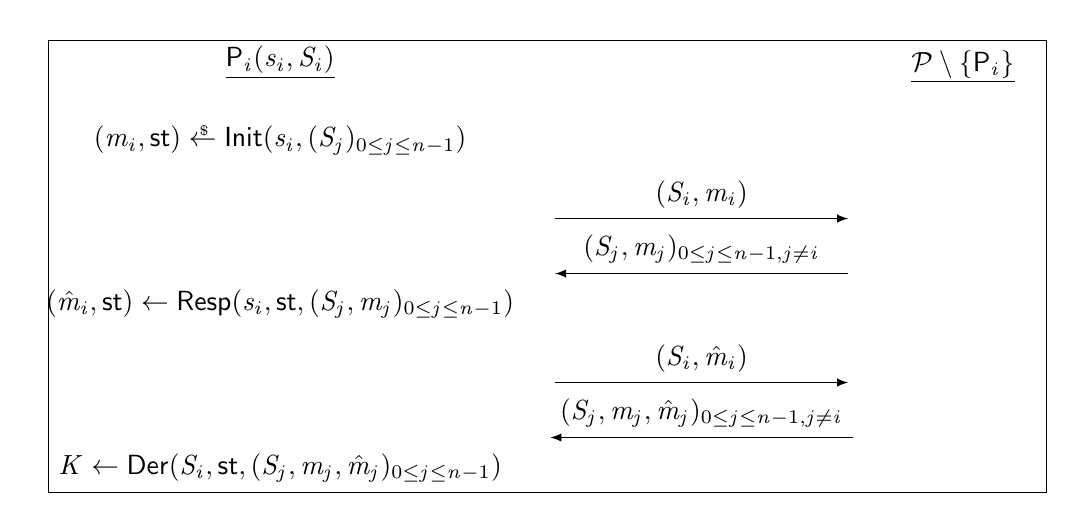
\begin{tikzpicture}
	\matrix (m)[matrix of nodes, column  sep=1em,row  sep=1mm,%
	column 2/.style={minimum width={width(" $(\spk_j,m_j,\hat{m}_j)_{0\leq j \leq n-1,j\neq i}$")},anchor=center},% 
	column 3/.style={minimum width=6em,anchor=center} ]{
		%line 1
	\underline{$\User[i](\ssk_i, \spk_i)$}& & \underline{$\PartySet\setminus\{\User[i]\}$} \\[2mm]
	%line 2
		$(m_i,\st) \getsr \GAKEIni (\ssk_i,(\spk_j)_{0\leq j \leq n-1})$ & &\\
	%line 3
		& $(\spk_i,m_i)$ & \\
	%line 4
		& $(\spk_j,m_j)_{0\leq j \leq n-1,j\neq i}$ & \\
	%line 5
		$(\hat{m}_i,\st) \gets \GAKERes(\ssk_i,\st,(\spk_j,m_j)_{0\leq j \leq n-1})$ & & \\ 
	%line 6
		& $(\spk_i,\hat{m}_i)$ & \\
	%line 7
		& $(\spk_j,m_j,\hat{m}_j)_{0\leq j \leq n-1,j\neq i}$ & \\
	%line 8
		$K \gets \GAKEDer (\spk_i,\st,(\spk_j,m_j,\hat{m}_j)_{0\leq j \leq n-1})$ & & \\ 
	};
	% drawing arrows
	\draw[-latex] (m-3-2.south west)--(m-3-2.south east);
	\draw[-latex] (m-4-2.south east)--(m-4-2.south west);
	\draw[-latex] (m-6-2.south west)--(m-6-2.south east);
	\draw[-latex] (m-7-2.south east)--(m-7-2.south west);
	\draw (m-8-1.south west) rectangle (m-1-3.north east);
	\end{tikzpicture}
		\caption{A $\GIAKE$ protocol flow from party $\User[i]$'s point of view. All messages (both sent and received ones) are broadcasted to all parties.}\label{fig:giakeprocedure}
\end{figure}

\subsection{Security model for GIAKE}\label{subsec:secmodel}
We now describe a security model for a two-round broadcast group authenticated key exchange, that allows a set of $n > 2$ parties to establish a common secret key.
The adversarial model is borrowed from \cite[Section 6.1]{PQR22}, which is in itself an extension to $\projectKey$ parties of the model described in \cite{JKRS20}.
Since we aim for implicit authentication for our 2-message protocol, we have to content ourselves with the notion of \textit{weak Forward Secrecy} (wFS), since no unsigned 2-message key-exchange protocol can hope for (full) Forward Secrecy \cite[Section 3.2]{HMQV}.
In particular, w.r.t. \cite[Section 6.1]{PQR22} we do not allow the adversary to actively participate in the session.\mattia{Argument: the adversary can act like party $\User[i]$ sending an ephemeral key of its choice, since it is unauthenticated. Then it reveals the long-term key of $\User[i]$ and computes the session key.}

\paragraph{Execution environment}



\subsection{Hash Proof System}\label{subsec:HPF}
We now recall the definitions of smooth projective hashing and hash proof system, introduced for the first time in \cite{CS02} and later picked up in \cite{JKRS20}.

Informally, a projective hash function is a keyed hash function associated with two types of keys: the secret \textit{hashing key}, which allows for hashing of every element in the domain, and a public \textit{projective key}, that can be used to hash only those elements that lie in a designated subset (the language) of the domain.
A projective hash function is \textit{smooth} if the projective key gives only a negligible advantage in correctly hashing an element that lies outside the designated subset.

\begin{definition}[Smooth projective hashing]
	Let $\Domain,\Codomain$ be two sets, let $\Language \subset \Domain$ be a language and let $\SKSpace,\PKSpace$ be the secret and public key spaces.
	For any secret key $\sk \in \SKSpace$, let $\Lambda_{\sk} : \Domain \rightarrow \Codomain$ be a keyed hash function.
	A hash function $\Lambda_{\sk}$ is \textbf{projective} if there exists a projection $\projectKey : \SKSpace \rightarrow \PKSpace$ such that the key $\pk = \projectKey(\sk)$ uniquely defines the action of $\Lambda_\sk$ on $\Language$: For every $\x \in \Language$, the digest $\y = \Lambda_\sk(\x)$ can be consistently computed from $\pk$ and $\x$.
	
	A projective hash function is \textbf{smooth} if, given any hashing key $\sk \getsr \SKSpace$ and its projection key $\pk = \projectKey(\sk)$, there exists only a negligible probability to successfully distinguish between samples from the distributions $D_1$ and $D_2$, where
	\[ D_1 := \{ (\x', \pk, \y) \mid \y = \Lambda_\sk(\x')) \}_{\x' \in \Domain\setminus\Language} \quad \text{and} \quad D_2 := \{(\x', \pk, \y) \mid \y \getsr \Codomain \}_{\x' \in \Domain\setminus\Language}\]
	Equivalently,\mattia{check this, I give a different definition here} let $\adv$ be an adversary that tries to compute the action of $\HPSHash_\sk$ on $\Domain \setminus \Language$ using the projection key $\pk = \projectKey(\sk)$ of a random $\sk \getsr \SKSpace$; then, for any $\x' \in \Domain \setminus \Language$,
	\[ \Pr \left[ \y \gets \adv(\pk,\x')  \mid \y = \HPSHash_\sk(\x') \right] \leq \negl[\secpar]\]\mattia{Possibly add the definition of $k$-entropic}
\end{definition}

Before moving on with the definition of a hash proof system, a few assumptions need to be made.
First, we assume that the projection function $\projectKey$ and the algorithms for sampling elements from $\Domain$ and from $\Language$ are efficient.
Secondly, we assume that for every $\x \in \Language$, one can efficiently produce a witness $w$ proving that $\x$ belongs to the language.

\begin{definition}
	A \textbf{Hash Proof System} (HPS) consists of three algorithms $\HPS = (\HPSParam,\HPSPrivEval,\HPSPubEval)$ defined as follows:
	\begin{itemize}
		\item $\HPSparams: = (\HPSgroup,\Codomain,\Domain,\Language,\SKSpace,\PKSpace,\HPSHash,\projectKey)  \getsr \HPSParam (1^\secpar)$: a PPT parameter setup algorithm that outputs a parameter set $\HPSparams$ containing a possibly empty set $\HPSgroup$ of extra parameters, a codomain $\Codomain$, a domain $\Domain$, a language $\Language$, a hashing key space $\SKSpace$, a projective key space $\PKSpace$, a smooth projective hash function $\HPSHash_{(\cdot)}: \Domain \rightarrow \Codomain$ and a projection function $\projectKey: \SKSpace \rightarrow \PKSpace$;
		\item $\y \gets \HPSPrivEval (\sk,\x)$: a deterministic private hashing algorithm that, on input a secret hashing key $\sk$ and an element $\x \in \Language$, outputs the digest $\y = \HPSHash_\sk(\x)$;
		\item $\y \gets \HPSPubEval (\pk,\x,w)$: a deterministic public hashing algorithm that, on input a projection key $\pk = \mu(\sk)$, an element $\x \in \Language$ and a witness $w$ for the fact that $\x \in \Language$, outputs the digest $\y = \HPSHash_\sk(\x)$.
	\end{itemize}
\end{definition}

The fundamental problem which an HPS bases its security on is the $m$- fold subset membership problem, which asks to tell elements sampled from the language apart from elements sampled in its complement.
\begin{problem}[$m$-fold Subset Membership Problem]
	Given $m$ elements uniformly drawn from $\Language$ and $m$ elements uniformly drawn from $\Domain \setminus \Language$, an adversary $\adv$ has a negligible advantage in distinguishing them; more formally,
	\begin{align*} \AdvSMP :=  & \big| \Pr \left[ 1 \gets \adv(\Domain,\Language,\x_1,\dots,\x_m )  \mid \x_1,\dots,\x_m \getsr \Language \right] - \\
		&\Pr \left[ 1 \gets \adv(\Domain,\Language,\x_1',\dots,\x_m' )  \mid \x_1',\dots,\x_m' \getsr \Domain \setminus \Language \right] \big| \leq \negl[\secpar] 
		\end{align*}
\end{problem}



	\section{Protocol}\label{sec:protocol}
Here is our new protocol.
	\section{Security}\label{sec:security}
We show our protocol secure.
	\section{Conclusions}\label{sec:conclusions}
We achieve something great.
Deal with it and publish our paper.
	
	\bibliographystyle{splncs03}
	\bibliography{cryptobib/abbrev3,cryptobib/crypto,add}
%	\bibliography{abbrev0,bibliography}
	
\end{document}
